\chapter{RESULTS}
\label{ch:results}

This chapter is divided into two main sections. The first section focuses on the comparison of the two motion correction techniques. The second section focuses on the results of the machine learning algorithms applied to the metrics extracted from the images.


\section{Simulated Data}

\subsection{Volume Registration: Power Thresholds}

% FD 150
\begin{figure}[t]
	\begin{subfigure}{0.45\textwidth}
		\centering
		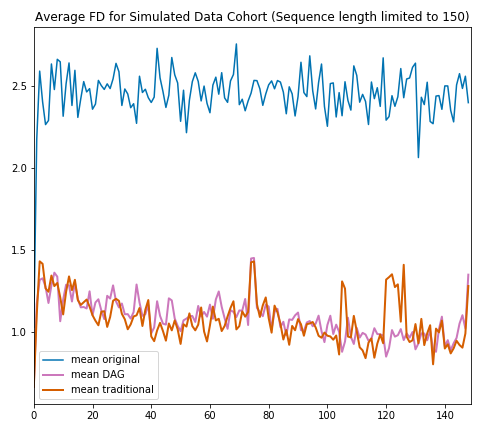
\includegraphics[width=1\textwidth]{6/figures/spectr_fd_all_150_avg.png}
		\caption{The average FD for all simulated images.}
	\end{subfigure}%	
	\vspace{0.1\textwidth}
	\begin{subfigure}{0.45\textwidth}
		\centering
		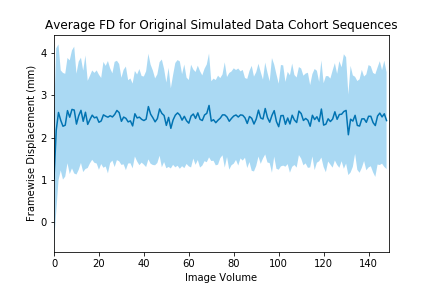
\includegraphics[width=1\textwidth]{6/figures/spectr-bold-fd-150.png}
		\caption{The mean and standard deviation of the FD for the original simulated images.}
	\end{subfigure}
	
	\begin{subfigure}{0.45\textwidth}
		\centering
		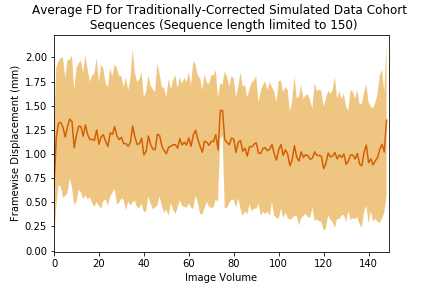
\includegraphics[width=1\textwidth]{6/figures/spectr-trad-fd-150.png}
		\caption{The mean and standard deviation of the FD for the simulated images registered using the traditional registration.}
	\end{subfigure}%	
	\vspace{0.1\textwidth}
	\begin{subfigure}{0.45\textwidth}
		\centering
		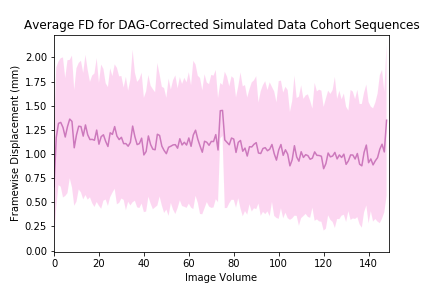
\includegraphics[width=1\textwidth]{6/figures/spectr-dag-fd-150.png}
		\caption{The mean and standard deviation of the FD for the simulated images registered using the DAG-based registration.}
	\end{subfigure}
\caption{The mean and standard deviations of the FD metrics distributions for all simulated images.}
\label{fig:spectr-fd-150}
\end{figure}

% DVARS 150
\begin{figure}[t]
	\begin{subfigure}{0.45\textwidth}
		\centering
		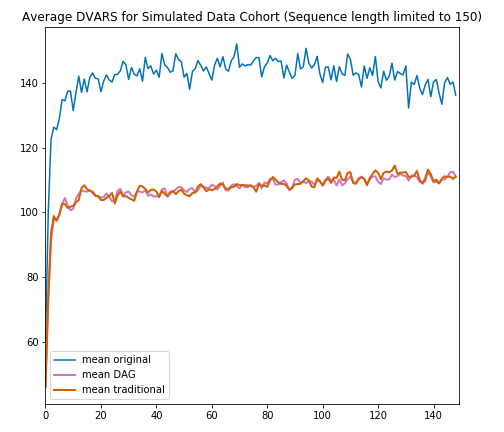
\includegraphics[width=1\textwidth]{6/figures/spectr_dvars_all_150_avg.png}
		\caption{The average DVARS for all simulated images.}
	\end{subfigure}%	
	\vspace{0.1\textwidth}
	\begin{subfigure}{0.45\textwidth}
		\centering
		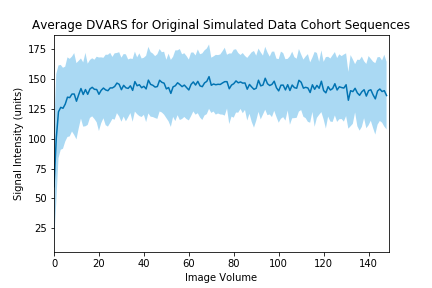
\includegraphics[width=1\textwidth]{6/figures/spectr-bold-dvars-150.png}
		\caption{The mean and standard deviation of the DVARS for the original simulated images.}
	\end{subfigure}
	
	\begin{subfigure}{0.45\textwidth}
		\centering
		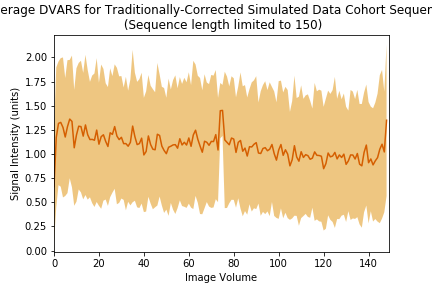
\includegraphics[width=1\textwidth]{6/figures/spectr-trad-dvars-150.png}
		\caption{The mean and standard deviation of the DVARS for the simulated images registered using the traditional registration.}
	\end{subfigure}%	
	\vspace{0.1\textwidth}
	\begin{subfigure}{0.45\textwidth}
		\centering
		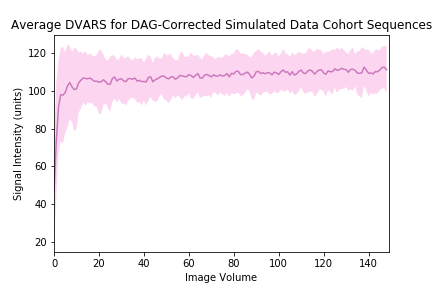
\includegraphics[width=1\textwidth]{6/figures/spectr-dag-dvars-150.png}
		\caption{The mean and standard deviation of the DVARS for the simulated images registered using the DAG-based registration.}
	\end{subfigure}
\caption{The mean and standard deviations of the DVARS metrics distributions for all simulated images.}
\label{fig:spectr-dvars-150}
\end{figure}

The FD and DVARS metrics were calculated between every pair of image volumes $i-1$ and $i$ for the original sequences and both types of registered sequences. The mean of the FD and DVARS metrics for each time point for each sequence type  can be seen in Figures

\begin{table}[]
\centering
\caption{The number and percentage of image volumes across all sequences in the simulated cohort which meet the usability thresholds of FD \textless 0.2 mm and DVARS \textless 2.5\%.}
\label{tab:spectr-power-thresh}
\begin{tabular}{|c|c|c|c|}
\hline
\textbf{Threshold Met} &
  \textbf{\begin{tabular}[c]{@{}c@{}}Original\\  Sequences\end{tabular}} &
  \textbf{\begin{tabular}[c]{@{}c@{}}Traditionally Registered \\ Sequences\end{tabular}} &
  \textbf{\begin{tabular}[c]{@{}c@{}}DAG-Registered \\ Sequences\end{tabular}} \\ \hline
FD (count)    & 98    & 329   & 279   \\ \hline
DVARS (count) & 54    & 53    & 53    \\ \hline
Both (count)  & 53    & 46    & 44    \\ \hline
FD (\%)       & 0.731 & 2.453 & 2.081 \\ \hline
DVARS(\%)     & 0.403 & 0.395 & 0.395 \\ \hline
Both (\%)     & 0.395 & 0.343 & 0.328 \\ \hline
\end{tabular}
\end{table}

Table \ref{tab:spectr-power-thresh} shows the number of and percentage of image volumes in all simulated image sequences which meet the FD threshold, the DVARS threshold, and both thresholds. Across all 90 image sequences, there were 150 image volumes per sequence bringing the total number of image volumes to 13,410 image volumes. In the original images, less than 1\% of the image volumes met the individual thresholds with only 0.395\% of image volumes meeting both thresholds. After either registration, over 2\% of the image volumes meet the FD threshold.

\begin{table}[]
\centering
\caption{Results from the t-tests comparing the counts for the numbers of images meeting the FD, DVARS, and FD and DVARS thresholds for sequence type $S_1$ and sequence type $S_2$.}
\label{tab:spectr-power-ttest}
\begin{tabular}{|c|c|c|c|}
\hline
\textbf{Sequence Type 1 ($S_1$)} &
  \textbf{Original} &
  \textbf{Original} &
  \textbf{\begin{tabular}[c]{@{}c@{}}Traditionally \\ Registered\end{tabular}} \\ \hline
\textbf{Sequence Type 2 ($S_2$)} &
  \textbf{\begin{tabular}[c]{@{}c@{}}Traditionally\\ Registered\end{tabular}} &
  \textbf{\begin{tabular}[c]{@{}c@{}}DAG\\ Registered\end{tabular}} &
  \textbf{\begin{tabular}[c]{@{}c@{}}DAG\\ Registered\end{tabular}} \\ \hline
\begin{tabular}[c]{@{}c@{}}P($S_1$ and $S_2$ have \\ same FD counts)\end{tabular} &
  1.05 E -16 &
  4.49 E -11 &
  0.127 \\ \hline
\begin{tabular}[c]{@{}c@{}}P($S_1$ and $S_2$ have \\ same DVARS counts)\end{tabular} &
  0.941 &
  0.941 &
  1.0 \\ \hline
\begin{tabular}[c]{@{}c@{}}P($S_1$ and $S_2$ have \\ same FD and DVARS counts)\end{tabular} &
  0.590 &
  0.486 &
  0.872 \\ \hline
\end{tabular}
\end{table}

To determine the statistical significance of these differences, a series of independent 2 sample t-tests were performed. For each test, two types of sequences were chosen. The distributions of samples were the numbers of image volumes in each sequence meeting the usability threshold of interest. The null hypotheses for the t-tests were that the number of volumes meeting the threshold for each sequence type were the same and the alternative hypothesis was that this number was different. The results of these tests can be seen in Table \ref{tab:spectr-power-ttest}. The only statistically significant differences were for the number of image volumes meeting the FD threshold. The counts for the registered images each differed from the original images at $p < 0.005$ while the difference between the two registrations was not significant ($p = 0.127$).

\begin{table}[]
\centering
\caption{The number of subjects whose sequences of types $S_1$ and $S_2$ had different FD distributions.}
\label{tab:spectr-fd-kstest}
\begin{tabular}{|c|c|c|c|}
\hline
\textbf{\begin{tabular}[c]{@{}c@{}}\# Sequences Type 1 \\ ($S_1$)\end{tabular}} &
  \textbf{\begin{tabular}[c]{@{}c@{}}\# Sequences Type 2 \\ ($S_2$)\end{tabular}} &
  \textbf{\begin{tabular}[c]{@{}c@{}}\# Sequences where \\ p \textless 0.05\end{tabular}} &
  \textbf{\begin{tabular}[c]{@{}c@{}}\# Sequences where \\ p \textless 0.005\end{tabular}} \\ \hline
Original                                                            & \begin{tabular}[c]{@{}c@{}}Traditionally\\ Registered\end{tabular} & 90 & 90 \\ \hline
Original                                                            & \begin{tabular}[c]{@{}c@{}}DAG\\ Registered\end{tabular}           & 90 & 90 \\ \hline
\begin{tabular}[c]{@{}c@{}}Traditionally \\ Registered\end{tabular} & \begin{tabular}[c]{@{}c@{}}DAG\\ Registered\end{tabular}           & 40 & 27 \\ \hline
\end{tabular}
\end{table}

\begin{table}[]
\centering
\caption{The number of subjects whose sequences of types $S_1$ and $S_2$ had different DVARS distributions.}
\label{tab:spectr-dvars-kstest}
\begin{tabular}{|c|c|c|c|}
\hline
\textbf{\begin{tabular}[c]{@{}c@{}}\# Sequences Type 1 \\ ($S_1$)\end{tabular}} &
  \textbf{\begin{tabular}[c]{@{}c@{}}\# Sequences Type 2 \\ ($S_2$)\end{tabular}} &
  \textbf{\begin{tabular}[c]{@{}c@{}}\# Sequences where \\ p \textless 0.05\end{tabular}} &
  \textbf{\begin{tabular}[c]{@{}c@{}}\# Sequences where \\ p \textless 0.005\end{tabular}} \\ \hline
Original                                                            & \begin{tabular}[c]{@{}c@{}}Traditionally\\ Registered\end{tabular} & 90 & 90 \\ \hline
Original                                                            & \begin{tabular}[c]{@{}c@{}}DAG\\ Registered\end{tabular}           & 90 & 90 \\ \hline
\begin{tabular}[c]{@{}c@{}}Traditionally \\ Registered\end{tabular} & \begin{tabular}[c]{@{}c@{}}DAG\\ Registered\end{tabular}           & 3  & 0  \\ \hline
\end{tabular}
\end{table}

For a more general comparison, the FD and DVARS metrics for each subject were compared for each type of registration. These distributions of FD and DVARS values for the original, traditionally registered and DAG-registered sequences underwent pairwise comparisons using the Kolmogorov-Smirnov test which evaluates the difference between two probability distributions. 

Table \ref{tab:spectr-fd-kstest} shows the number of comparisons between each sequence type where the Kolmogorov-Smirnov test produced a p-value less than 0.05 and 0.005 for the FD metrics. This table shows that the all images registered using either type of registration had significantly different FD distributions than the original images. It also shows that the traditionally registered and DAG-registered sequences had significantly different FD distributions with $p < 0.05$ for almost half (40/90) of the sequences and $p < 0.005$ for almost a third (27/90) of the sequences.

Table \ref{tab:spectr-dvars-kstest} shows similar results for the DVARS metrics of the registered and original sequences. However, only 3/90 of the registered image sequences had different DVARS distributions at $p < 0.05$. 



%Independent 2 sample t-test
%Null hypothesis: number of Traditional and DAG registered images meeting the FD threshold are the same
%Alternative hypothesis: number of traditional and dag registered images meeting the FD threshold are different
%Gather data: get number of images meeting each threshold from each sequence

\subsection{Volume Registration: Sequence Duration Motion}

Motion across the whole sequence was measured by comparing every image volume in the sequence to every other image volume in the sequence. The three metrics used for this comparison were the correlation ratio, the Dice metric, and the mutual information. The calculations for metric on one sequence produced a two dimensional matrix of metric values. 

These matrices were used for two types of analysis. The first analysis was to compare the quantities of motion over the course of an entire sequence. The second analysis was to identify sequences containing similar patterns of motion throughout the duration of the sequence.

For the first analysis, the metrics matrices were compared to each other 

To compare motion patterns, the metrics matrices were normalized for each subject.


The differences in the motion patterns embodied by the normalized matrices were different between the original, traditionally registered, and DAG-registered sequences for each simulated subject was significant at $p < 0.005$.

Use t-test to compare the normalized matrices for all simulated subjects across a single registration type. Plot a clustermap based on 2 coordinates and the distance (p-value) between them

\section{Preadolescent Cohort}

\begin{table}[]
\centering
\caption{The number and percentage of image volumes across all sequences in the preadolescent cohort which meet the usability thresholds of FD \textless 0.2 mm and DVARS \textless 2.5\%.}
\label{tab:pread-power-thresh}
\begin{tabular}{|c|c|c|c|}
\hline
\textbf{Threshold Met} &
  \textbf{\begin{tabular}[c]{@{}c@{}}Original\\  Sequences\end{tabular}} &
  \textbf{\begin{tabular}[c]{@{}c@{}}Traditionally Registered \\ Sequences\end{tabular}} &
  \textbf{\begin{tabular}[c]{@{}c@{}}DAG-Registered \\ Sequences\end{tabular}} \\ \hline
FD (count)    & 107879 & 72104 & 72114 \\ \hline
DVARS (count) & 87169  & 54056 & 53756 \\ \hline
Both (count)  & 74107  & 45006 & 44682 \\ \hline
FD (\%)       & 60.17  & 40.22 & 40.26 \\ \hline
DVARS(\%)     & 48.62  & 30.15 & 30.01 \\ \hline
Both (\%)     & 41.33  & 25.10 & 24.94 \\ \hline
\end{tabular}
\end{table}

Table \ref{tab:pread-power-thresh} contains the number and percentages of image volumes from the whole preadolescent cohort which meet the FD and DVARS thresholds. 

\begin{table}[]
\centering
\caption{Results from the t-tests comparing the counts for the numbers of images meeting the FD, DVARS, and FD and DVARS thresholds for sequence type $S_1$ and sequence type $S_2$.}
\label{tab:pread-power-ttest}
\begin{tabular}{|c|c|c|c|}
\hline
\textbf{Sequence Type 1 ($S_1$)} &
  \textbf{Original} &
  \textbf{Original} &
  \textbf{\begin{tabular}[c]{@{}c@{}}Traditionally \\ Registered\end{tabular}} \\ \hline
\textbf{Sequence Type 2 ($S_2$)} &
  \textbf{\begin{tabular}[c]{@{}c@{}}Traditionally\\ Registered\end{tabular}} &
  \textbf{\begin{tabular}[c]{@{}c@{}}DAG\\ Registered\end{tabular}} &
  \textbf{\begin{tabular}[c]{@{}c@{}}DAG\\ Registered\end{tabular}} \\ \hline
\begin{tabular}[c]{@{}c@{}}P($S_1$ and $S_2$ have \\ same FD counts)\end{tabular} &
  2.81 E -16 &
  2.35 E -16 &
  0.998 \\ \hline
\begin{tabular}[c]{@{}c@{}}P($S_1$ and $S_2$ have \\ same DVARS counts)\end{tabular} &
  9.43 E -12 &
  5.30 E -12 &
  0.950 \\ \hline
\begin{tabular}[c]{@{}c@{}}P($S_1$ and $S_2$ have \\ same FD and DVARS counts)\end{tabular} &
  1.12 E -11 &
  5.60 E -12 &
  0.938 \\ \hline
\end{tabular}
\end{table}

Table \ref{tab:pread-power-ttest} shows the results of a set of t-tests which determine if the distribution of metric X for sequence type $S_1$ is the same as the distribution of metric X for sequence type $S_2$.

\begin{table}[]
\centering
\caption{The number of subjects whose sequences of types $S_1$ and $S_2$ had different FD distributions.}
\label{tab:power-fd-kstest}
\begin{tabular}{|c|c|c|c|}
\hline
\textbf{\begin{tabular}[c]{@{}c@{}}\# Sequences Type 1 \\ ($S_1$)\end{tabular}} &
  \textbf{\begin{tabular}[c]{@{}c@{}}\# Sequences Type 2 \\ ($S_2$)\end{tabular}} &
  \textbf{\begin{tabular}[c]{@{}c@{}}\# Sequences where \\ p \textless 0.05\end{tabular}} &
  \textbf{\begin{tabular}[c]{@{}c@{}}\# Sequences where \\ p \textless 0.005\end{tabular}} \\ \hline
Original                                                            & \begin{tabular}[c]{@{}c@{}}Traditionally\\ Registered\end{tabular} & 331 & 326 \\ \hline
Original                                                            & \begin{tabular}[c]{@{}c@{}}DAG\\ Registered\end{tabular}           & 332 & 328 \\ \hline
\begin{tabular}[c]{@{}c@{}}Traditionally \\ Registered\end{tabular} & \begin{tabular}[c]{@{}c@{}}DAG\\ Registered\end{tabular}           & 19 &17 \\ \hline
\end{tabular}
\end{table}

\begin{table}[]
\centering
\caption{The number of subjects whose sequences of types $S_1$ and $S_2$ had different DVARS distributions.}
\label{tab:power-dvars-kstest}
\begin{tabular}{|c|c|c|c|}
\hline
\textbf{\begin{tabular}[c]{@{}c@{}}\# Sequences Type 1 \\ ($S_1$)\end{tabular}} &
  \textbf{\begin{tabular}[c]{@{}c@{}}\# Sequences Type 2 \\ ($S_2$)\end{tabular}} &
  \textbf{\begin{tabular}[c]{@{}c@{}}\# Sequences where \\ p \textless 0.05\end{tabular}} &
  \textbf{\begin{tabular}[c]{@{}c@{}}\# Sequences where \\ p \textless 0.005\end{tabular}} \\ \hline
Original                                                            & \begin{tabular}[c]{@{}c@{}}Traditionally\\ Registered\end{tabular} & 334 & 331 \\ \hline
Original                                                            & \begin{tabular}[c]{@{}c@{}}DAG\\ Registered\end{tabular}           & 334 & 333 \\ \hline
\begin{tabular}[c]{@{}c@{}}Traditionally \\ Registered\end{tabular} & \begin{tabular}[c]{@{}c@{}}DAG\\ Registered\end{tabular}           & 22  & 19  \\ \hline
\end{tabular}
\end{table}

%-----------------------------------------------------------------
\section{Neonatal Cohort}

\begin{table}[]
\centering
\caption{The number and percentage of image volumes across all sequences in the neonatal cohort which meet the usability thresholds of FD \textless 0.2 mm and DVARS \textless 2.5\%.}
\label{tab:neonate-power-thresh}
\begin{tabular}{|c|c|c|c|}
\hline
\textbf{Threshold Met} &
  \textbf{\begin{tabular}[c]{@{}c@{}}Original\\  Sequences\end{tabular}} &
  \textbf{\begin{tabular}[c]{@{}c@{}}Traditionally Registered \\ Sequences\end{tabular}} &
  \textbf{\begin{tabular}[c]{@{}c@{}}DAG-Registered \\ Sequences\end{tabular}} \\ \hline
FD (count)    & 16495  & 14264 & 14173 \\ \hline
DVARS (count) & 16820  & 13903 & 13752 \\ \hline
Both (count)  & 15332  & 12837 & 12684 \\ \hline
FD (\%)       & 69.59  & 60.18 & 59.79 \\ \hline
DVARS(\%)     & 70.96  & 58.65 & 58.02 \\ \hline
Both (\%)     & 64.68  & 54.16 & 53.51 \\ \hline
\end{tabular}
\end{table}

Table \ref{tab:neonate-power-thresh} contains the number and percentages of image volumes from the whole neonatal cohort which meet the FD and DVARS thresholds. The total number of image volumes in across all sequences of a single type was 23704.

\begin{table}[]
\centering
\caption{Results from the t-tests comparing the counts for the numbers of images meeting the FD, DVARS, and FD and DVARS thresholds for sequence type $S_1$ and sequence type $S_2$.}
\label{tab:neonate-power-ttest}
\begin{tabular}{|c|c|c|c|}
\hline
\textbf{Sequence Type 1 ($S_1$)} &
  \textbf{Original} &
  \textbf{Original} &
  \textbf{\begin{tabular}[c]{@{}c@{}}Traditionally \\ Registered\end{tabular}} \\ \hline
\textbf{Sequence Type 2 ($S_2$)} &
  \textbf{\begin{tabular}[c]{@{}c@{}}Traditionally\\ Registered\end{tabular}} &
  \textbf{\begin{tabular}[c]{@{}c@{}}DAG\\ Registered\end{tabular}} &
  \textbf{\begin{tabular}[c]{@{}c@{}}DAG\\ Registered\end{tabular}} \\ \hline
\begin{tabular}[c]{@{}c@{}}P($S_1$ and $S_2$ have \\ same FD counts)\end{tabular} &
  0.0110 &
  0.00813 &
  0.924 \\ \hline
\begin{tabular}[c]{@{}c@{}}P($S_1$ and $S_2$ have \\ same DVARS counts)\end{tabular} &
  0.00163 &
  0.000942 &
  0.880 \\ \hline
\begin{tabular}[c]{@{}c@{}}P($S_1$ and $S_2$ have \\ same FD and DVARS counts)\end{tabular} &
  0.00779 &
  0.00475 &
  0.879 \\ \hline
\end{tabular}
\end{table}

Table \ref{tab:neonate-power-ttest} shows the results of a set of t-tests which determine if the distribution of metric X for sequence type $S_1$ is the same as the distribution of metric X for sequence type $S_2$.

\begin{table}[]
\centering
\caption{The number of subjects whose sequences of types $S_1$ and $S_2$ had different FD distributions.}
\label{tab:neonate-fd-kstest}
\begin{tabular}{|c|c|c|c|}
\hline
\textbf{\begin{tabular}[c]{@{}c@{}}\# Sequences Type 1 \\ ($S_1$)\end{tabular}} &
  \textbf{\begin{tabular}[c]{@{}c@{}}\# Sequences Type 2 \\ ($S_2$)\end{tabular}} &
  \textbf{\begin{tabular}[c]{@{}c@{}}\# Sequences where \\ p \textless 0.05\end{tabular}} &
  \textbf{\begin{tabular}[c]{@{}c@{}}\# Sequences where \\ p \textless 0.005\end{tabular}} \\ \hline
Original                                                            & \begin{tabular}[c]{@{}c@{}}Traditionally\\ Registered\end{tabular} & 36	 & 32 \\ \hline
Original                                                            & \begin{tabular}[c]{@{}c@{}}DAG\\ Registered\end{tabular}           & 42 & 38 \\ \hline
\begin{tabular}[c]{@{}c@{}}Traditionally \\ Registered\end{tabular} & \begin{tabular}[c]{@{}c@{}}DAG\\ Registered\end{tabular}           & 13 & 5 \\ \hline
\end{tabular}
\end{table}

\begin{table}[]
\centering
\caption{The number of subjects whose sequences of types $S_1$ and $S_2$ had different DVARS distributions.}
\label{tab:neonate-dvars-kstest}
\begin{tabular}{|c|c|c|c|}
\hline
\textbf{\begin{tabular}[c]{@{}c@{}}\# Sequences Type 1 \\ ($S_1$)\end{tabular}} &
  \textbf{\begin{tabular}[c]{@{}c@{}}\# Sequences Type 2 \\ ($S_2$)\end{tabular}} &
  \textbf{\begin{tabular}[c]{@{}c@{}}\# Sequences where \\ p \textless 0.05\end{tabular}} &
  \textbf{\begin{tabular}[c]{@{}c@{}}\# Sequences where \\ p \textless 0.005\end{tabular}} \\ \hline
Original                                                            & \begin{tabular}[c]{@{}c@{}}Traditionally\\ Registered\end{tabular} & 44 & 39 \\ \hline
Original                                                            & \begin{tabular}[c]{@{}c@{}}DAG\\ Registered\end{tabular}           & 45 & 44 \\ \hline
\begin{tabular}[c]{@{}c@{}}Traditionally \\ Registered\end{tabular} & \begin{tabular}[c]{@{}c@{}}DAG\\ Registered\end{tabular}           & 11  & 5  \\ \hline
\end{tabular}
\end{table}

\section{Comparison of Volume Registration Methods}

\subsection{Overview}

Each of the clinical images underwent volume registration using both registration methods outlined in Chapter \ref{ch:moco}. The FD and DVARs metrics were calculated for every pair of subsequent volumes $i$ and $i+1$ in the original sequences, the traditionally registered sequences, and the DAG-registered sequences. Then the sequences were comprehensively compared to themselves. For every volume in each sequence, the Dice metric, the mutual information, and the correlation ratio were calculated for the volume and every other volume in the sequence.

The simulated data underwent the same analyses as the clinical images, with one addition. Independent component analysis was performed on the simulated data to identify components contributing to the overall signal in the image. By correlating the components with the simulated signal for each image, the BOLD-related components were identifies. The amount of BOLD signal identified for each image was compared to that image's original BOLD signal.

\subsection{Neonatal Cohort}

(Still processing.)

\subsection{Preadolescent Cohort}




% First: FD and DVARs
The averages of the distributions of the FD and DVARs metrics across the whole time period of the sequences for the original, traditionally registered, and DAG-registered images were calculated. The images sequences varied in length from 150 volume to 450 volumes due to the differences in acquisition protocols at different sites. The means and standard deviations of FD and DVARS metrics for the entire set of sequence with their original lengths can be seen in Figures \ref{fig:pread-fd-450} and \ref{fig:pread-dvars-450}. The means and standard deviations of the FD and DVARs metrics for the first 150 volumes in each sequence can be seen in Figures \ref{fig:pread-dvars-150} and \ref{fig:pread-dvars-150}. 

% FD 450
\begin{figure}[t]
	\centering
	\begin{subfigure}{0.8\textwidth}
		\centering
		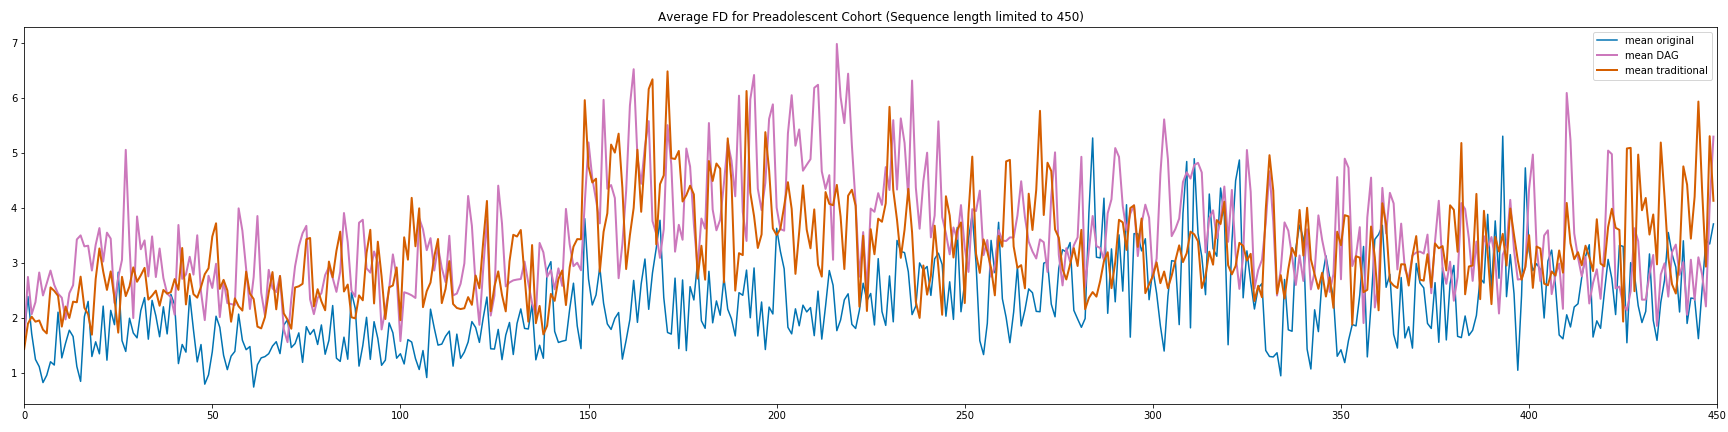
\includegraphics[width=1.0\textwidth]{6/figures/pread_fd_all_450_avg.png}
		\caption{The average FD of all preadolescent images.}
	\end{subfigure}

	\begin{subfigure}{0.9\textwidth}
		\centering
		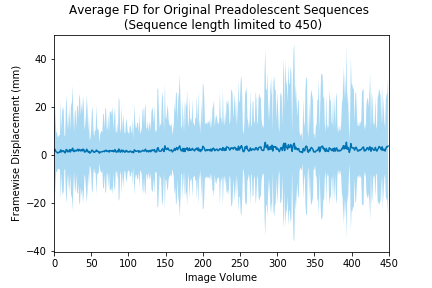
\includegraphics[width=.4\textwidth]{6/figures/pread-bold-fd-450.png}
		\caption{The mean and standard deviation of the FD for the original images.}
	\end{subfigure}
	
	\begin{subfigure}{0.9\textwidth}
		\centering
		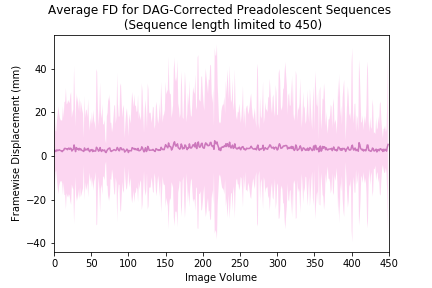
\includegraphics[width=0.4\textwidth]{6/figures/pread-dag-fd-450.png}
		\caption{The mean and standard deviation of the FD for the DAG-corrected images.}
	\end{subfigure}
	
	\begin{subfigure}{0.9\textwidth}
		\centering
		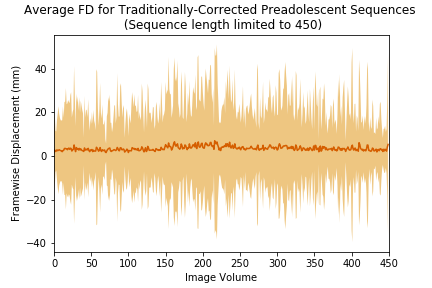
\includegraphics[width=0.4\textwidth]{6/figures/pread-trad-fd-450.png}
		\caption{The mean and standard deviation of the FD for the DAG-corrected images.}
	\end{subfigure}
\caption{The FD distributions for all preadolescent images, with sequence length limited to 450 volumes.}
\label{fig:pread-fd-450}
\end{figure}

% FD 150
\begin{figure}[t]
	\centering
	\begin{subfigure}{0.45\textwidth}
		\centering
		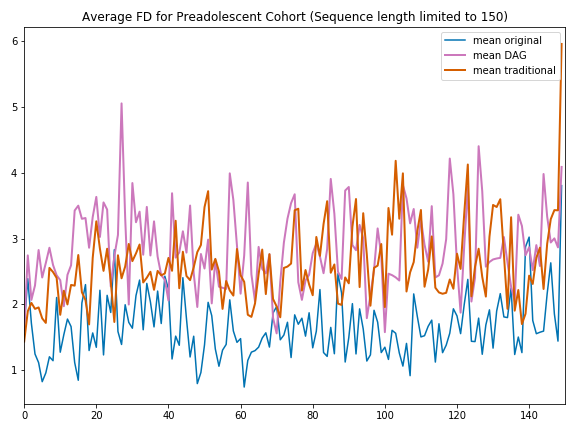
\includegraphics[width=1\textwidth]{6/figures/pread_fd_all_150_avg.png}
		\caption{The average FD of all preadolescent images.}
	\end{subfigure}%
	\vspace{0.05\textwidth}
	\begin{subfigure}{0.45\textwidth}
		\centering
		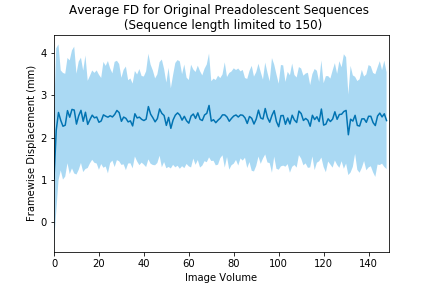
\includegraphics[width=1\textwidth]{6/figures/pread-bold-fd-150.png}
		\caption{The mean and standard deviation of the FD for the original images.}
	\end{subfigure}
	
	\begin{subfigure}{0.45\textwidth}
		\centering
		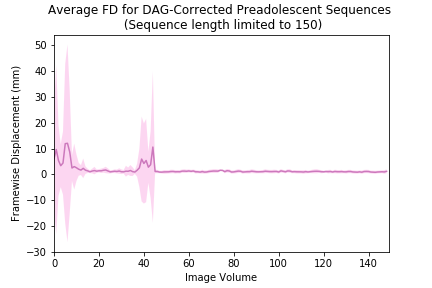
\includegraphics[width=1\textwidth]{6/figures/pread-dag-fd-150.png}
		\caption{The mean and standard deviation of the FD for the DAG-corrected images.}
	\end{subfigure}%	
	\vspace{0.05\textwidth}
	\begin{subfigure}{0.45\textwidth}
		\centering
		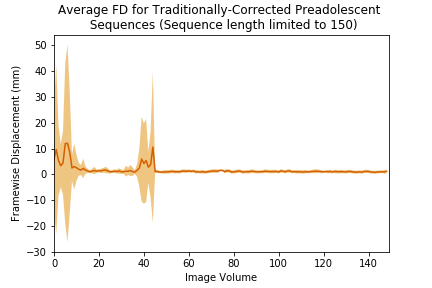
\includegraphics[width=1\textwidth]{6/figures/pread-trad-fd-150.png}
		\caption{The mean and standard deviation of the FD for the DAG-corrected images.}
	\end{subfigure}
\caption{The FD distributions for all preadolescent images, with sequence length limited to the minimum of 150 volumes.}
\label{fig:pread-fd-150}
\end{figure}

% DVARS 450
\begin{figure}[t]
	\centering
	\begin{subfigure}{0.9\textwidth}
		\centering
		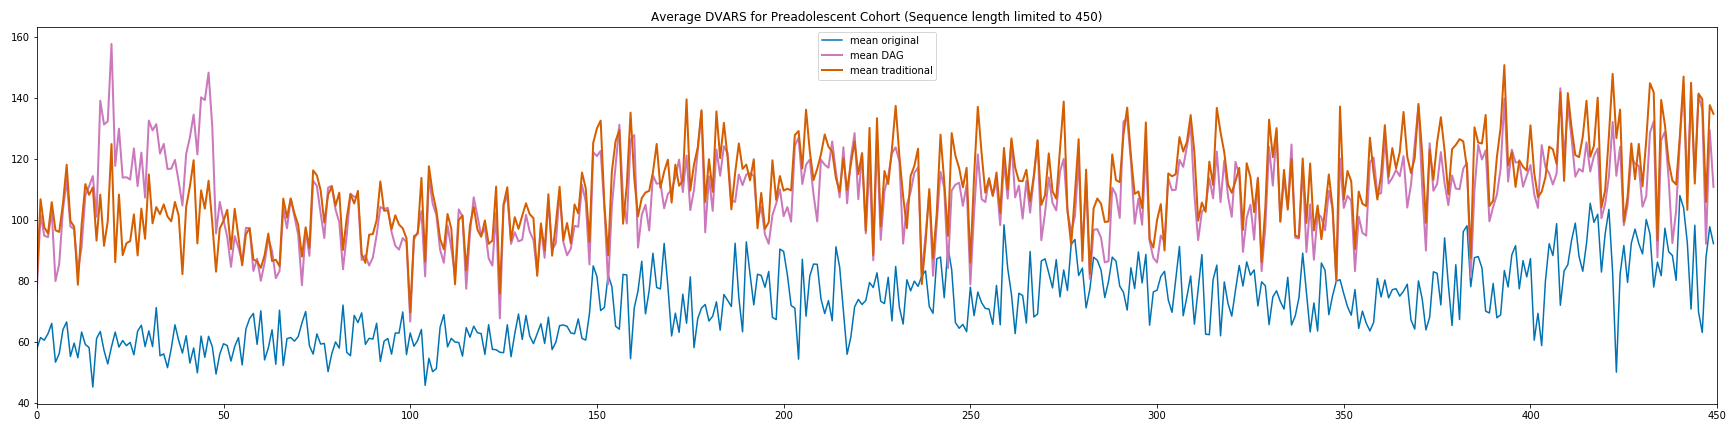
\includegraphics[width=1.0\textwidth]{6/figures/pread_dvars_all_450_avg.png}
		\caption{The average DVARS of all preadolescent images.}
	\end{subfigure}

	\begin{subfigure}{0.9\textwidth}
		\centering
		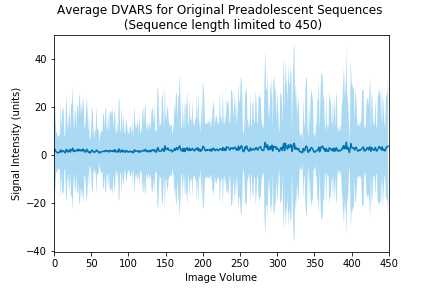
\includegraphics[width=.4\textwidth]{6/figures/pread-bold-dvars-450.png}
		\caption{The mean and standard deviation of the DVARS for the original images.}
	\end{subfigure}
	
	\begin{subfigure}{0.9\textwidth}
		\centering
		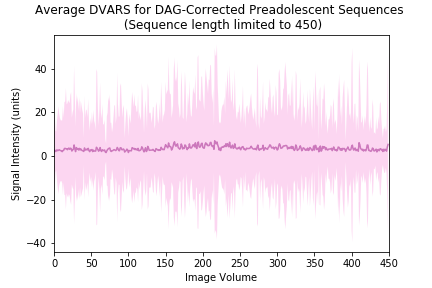
\includegraphics[width=0.4\textwidth]{6/figures/pread-dag-dvars-450.png}
		\caption{The mean and standard deviation of the DVARS for the DAG-corrected images.}
	\end{subfigure}
	
	\begin{subfigure}{0.9\textwidth}
		\centering
		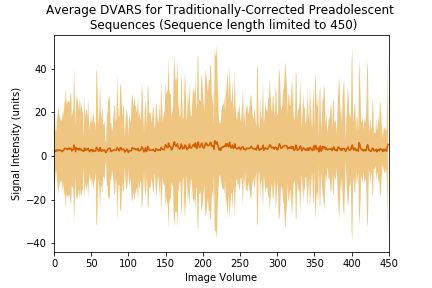
\includegraphics[width=0.4\textwidth]{6/figures/pread-trad-dvars-450.png}
		\caption{The mean and standard deviation of the DVARS for the DAG-corrected images.}
	\end{subfigure}
\caption{The DVARS distributions for all preadolescent images, with sequence length limited to 450 volumes.}
\label{fig:pread-dvars-450}
\end{figure}

% DVARS 150
\begin{figure}[t]
	\centering
	\begin{subfigure}{0.45\textwidth}
		\centering
		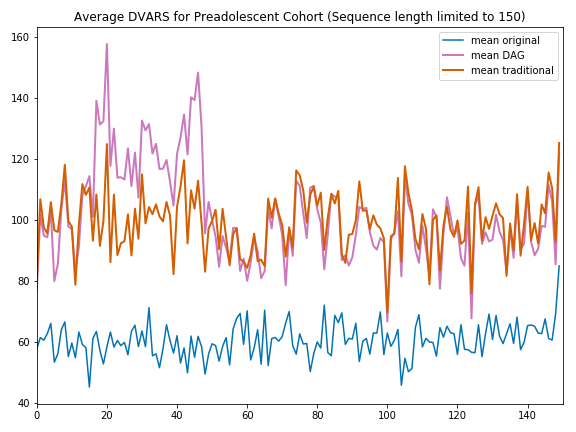
\includegraphics[width=1\textwidth]{6/figures/pread_dvars_all_150_avg.png}
		\caption{The average DVARS of all preadolescent images.}
	\end{subfigure}%
	\vspace{0.05\textwidth}
	\begin{subfigure}{0.45\textwidth}
		\centering
		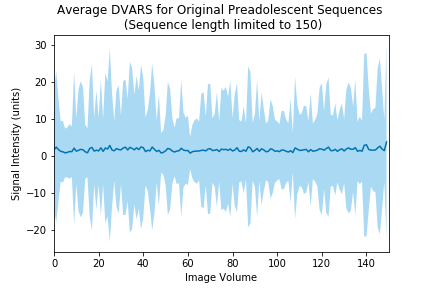
\includegraphics[width=1\textwidth]{6/figures/pread-bold-dvars-150.png}
		\caption{The mean and standard deviation of the DVARS for the original images.}
	\end{subfigure}
	
	\begin{subfigure}{0.45\textwidth}
		\centering
		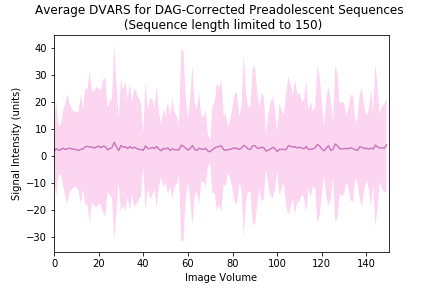
\includegraphics[width=1\textwidth]{6/figures/pread-dag-dvars-150.png}
		\caption{The mean and standard deviation of the DVARS for the DAG-corrected images.}
	\end{subfigure}%	
	\vspace{0.05\textwidth}
	\begin{subfigure}{0.45\textwidth}
		\centering
		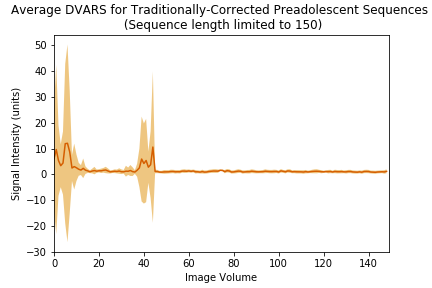
\includegraphics[width=1\textwidth]{6/figures/pread-trad-dvars-150.png}
		\caption{The mean and standard deviation of the DVARS for the DAG-corrected images.}
	\end{subfigure}
\caption{The DVARS distributions for all preadolescent images, with sequence length limited to the minimum of 150 volumes.}
\label{fig:pread-dvars-150}
\end{figure}

To compare the FD and DVARS values for each type of motion correction, the metrics for each image were considered to be independent samples drawn from an unknown distribution. Pairwise comparisons of these distribution were performed using the Kolmogorov-Smirnov (KS) test. The two-sided KS test measures the distance between the empirical distributions of two distributions. The null hypothesis of the two-sided KS test is that the empirical distributions being compared come from the same underlying distribution. As the KS test is nonparametric, the metrics for all image volumes can be used.

By comparing the distributions for the original sequences to the distributions for the registered sequences, we aim to determine if the volume registration had a significant effect on the images themselves. The comparison of the distributions for the two types of registered images is intended to determine if there is a statistically significant difference between the FD and DVARS distributions of the registered images.

\begin{table}[ht]
\centering
\caption{The KS test statistics and p-values for the KS test comparisons of FD values for the preadolescent cohort.}
\label{tab:pread-ks-fd}
\begin{tabular}{|l|c|c|}
\hline
\textbf{Pair of Image Types} & \multicolumn{1}{l|}{\textbf{KS Statistic}} & \multicolumn{1}{l|}{\textit{\textbf{p-value}}} \\ \hline
Original and DAG Registered                 & 0.34707   & 0.0     \\ \hline
Original and Traditionally Registered       & 0.34792   & 0.0     \\ \hline
DAG Registered and Traditionally Registered & 0.0023160 & 0.52633 \\ \hline
\end{tabular}
\end{table}

\begin{table}[ht]
\centering
\caption{The KS test statistics and p-values for the KS test comparisons of DVARS values for the preadolescent cohort.}
\label{tab:pread-ks-dvars}
\begin{tabular}{|l|c|c|}
\hline
\textbf{Pair of Image Types} & \multicolumn{1}{l|}{\textbf{KS Statistic}} & \multicolumn{1}{l|}{\textit{\textbf{p-value}}} \\ \hline
Original and DAG Registered                 & 0.38692   & 0.0     \\ \hline
Original and Traditionally Registered       & 0.38699   & 0.0     \\ \hline
DAG Registered and Traditionally Registered & 0.0024913 & 0.43193 \\ \hline
\end{tabular}
\end{table}

The KS statistic and p-value produced as result of the KS tests can be seen in Table \ref{tab:pread-ks-fd} for the FD metrics and in Table \ref{tab:pread-ks-dvars} for the DVARS metrics.


%Each rs-fMRI sequence in the cohort underwent registration using both frameworks. For each sequence, the correlation ratio between every possible pair of volumes was calculated. A set of metrics of the correlation ratio matrices for each sequence can be seen in Table \ref{tab:crm-stats}. This table shows that the original sequences generally have higher average correlation ratios and contain more variation in their correlation ratios than the globally registered images. The registration methods were able to reduce the mean and variability of the correlation ratios across all subjects in the cohort who had original correlation ratio averages of at least 0.035.

\begin{table}[ht]
\centering
\caption{The number of and percentage of images from each category which met the FD and DVARS thresholds.}
\label{tab:pread-powerthresh}
\begin{tabular}{|c|c|c|c|}
\hline
\textbf{Thresholds Met} &
  \textbf{\begin{tabular}[c]{@{}c@{}}Original \\ Images\end{tabular}} &
  \textbf{\begin{tabular}[c]{@{}c@{}}DAG-Registered \\ Images\end{tabular}} &
  \textbf{\begin{tabular}[c]{@{}c@{}}Traditionally-Registered\\  Images\end{tabular}} \\ \hline
FD (count)           & 107896 & 28998  & 28761  \\ \hline
DVARS (count)        & 87169  & 11445  & 11375  \\ \hline
FD and DVARS (count) & 74112  & 9289   & 9257   \\ \hline
FD (\%)              & 60.178 & 16.189 & 16.041 \\ \hline
DVARS (\%)           & 48.618 & 6.389  & 6.344  \\ \hline
FD and DVARS (\%)    & 41.335 & 5.185  & 5.163  \\ \hline
\end{tabular}
\end{table}


The FD and DVARS values were compared to the usability thresholds defined by Power et al. to determine how many volumes were recovered by each framework \cite{Power2014}. Table \ref{tab:pread-powerthresh} shows the number of volumes meeting each threshold, both in terms of the number of volumes in the cohort and the percentage of volumes in the cohort. In the original dataset, almost 42\% of image volumes met both the FD and DVARS thresholds. However, only about 5\% of volumes met both thresholds for each registration type. Looking at the thresholds independently, about 60\% of volumes met the FD threshold before registration and only 16\% of volumes met the threshold after registration. Similarly, about 48\% of volumes met the DVARS threshold before registration and only about 6\% of volumes met the threshold after registration. These results suggest that the registration process introduces some degree of error into the preadolescent images, at least with respect to the established usability criteria.

\begin{figure}[ht]
\centering
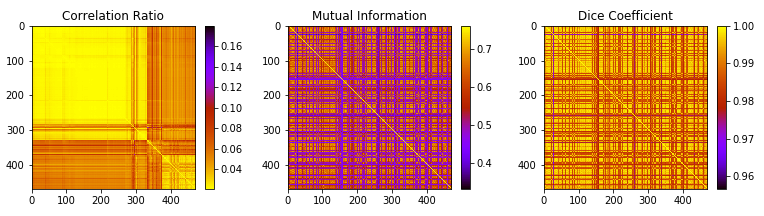
\includegraphics[width=1\textwidth]{6/figures/similarity-mat-sample.png}
\caption{Examples of the three similarity matrices. Lighter colors represent more desirable values.}
\label{fig:sim-mat-sample}
\end{figure}

An example of the three similarity matrices can be seen in Figure \ref{fig:sim-mat-sample}. The element $e_{i,j}$ represents the value of the given metric between the image volumes represented by row $i$ and column $j$. Each metric measures similarity according to slightly different definitions. In this figure, lighter values represent better metric values while darker values indicate lower similarity.

It is important to note the scales for these three metrics vary. The correlation ratio measures the distance between two items. Lower values for the correlation ratio means there is a smaller distance between the given pair of image volumes. The mutual information measures the shared information between two distributions of samples which may or may not be generated from the same underlying distribution. Higher mutual information values mean more shared information and low values mean less shared information. The Dice coefficient measures the overlap of two binary images. High Dice coefficients indicate a large amount of overlap, with a value of 1.0 indicating a perfect overlap.

The correlation ratio matrix in Figure \ref{fig:sim-mat-sample} suggests that the patient remained relatively still for the first 300 volumes of the image, then moved for about 100 volumes, and remained still in a new position for the last 50 frames of the sequence. The colors representing the correlation ratios correspond to very low values, suggesting there is little patient motion overall.

The Dice coefficient matrix has a similar pattern as the mutual information matrix, but leads to a different conclusion. The Dice coefficient was calculated on an Otsu thresholded version of each image volume. As the values of the Dice coefficients are consistently high, the patient likely did not move much. 

The mutual information matrix shows that the shared information throughout the entire image sequence varies. Using the information from the correlation ratio matrix and the Dice coefficient matrix, it is possible that the variations in the mutual information matrix are due to changes in the rs-fMRI signal caused by BOLD signal changes, spin history effects of motion, and susceptibility effects of motion.


\subsection{Fetal Cohort}

(Still processing.)

\subsection{Simulated Images}


\section{Motion Patterns}
